% Research Idea 3 section for the 11-777 midterm report (ICML 2026 template).
% Paste into main.tex in place of the "Research Idea 3" section; needs \usepackage{amsmath,amssymb}
% and fig_idea3_pipeline.pdf next to main.tex. Bib entries are in idea3_refs.bib.
% Every number below comes from idea3_consistency/results_* (job ids given in the text).

\section{Research Idea 3: Answer-Preserving Transformations as a Probe of Spatial Grounding}
\label{sec:idea3}

\begin{figure*}[t]
  \centering
  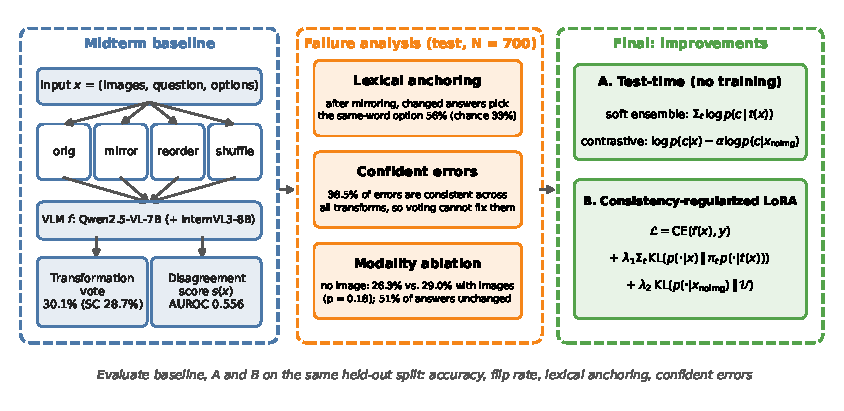
\includegraphics[width=\textwidth]{fig_idea3_pipeline.pdf}
  \caption{Overview of Research Idea 3. \textbf{Left:} each question is paired with
  answer-preserving variants (image mirroring with left/right words swapped, image reordering,
  option shuffling) and the VLM's answers are compared. \textbf{Middle:} the three main failure
  modes found on the held-out test split. \textbf{Right:} the test-time and training-time
  improvements we propose for the final report.}
  \label{fig:idea3-overview}
\end{figure*}

\subsection{Initial Implementation}

\paragraph{Setup.}
A question in MMSI-Bench~\citep{yang2025mmsi} is $x=(I_1,\dots,I_m,q,o_A,\dots,o_D)$, with
$m\ge 2$ images, a question $q$, four options and a gold letter $y$. A VLM with parameters
$\theta$ gives $p_\theta(c\mid x)$ over letters $c\in\mathcal{C}=\{A,B,C,D\}$, and we use its
greedy answer $\hat y(x)=\arg\max_c p_\theta(c\mid x)$. We call a transformation $t$
\emph{answer-preserving} if there is a known bijection $\pi_t:\mathcal{C}\to\mathcal{C}$ with
$y(t(x))=\pi_t(y(x))$. We use three:
\begin{itemize}
  \item \textbf{mirror}: flip every image horizontally and swap left$\leftrightarrow$right
  (and clockwise$\leftrightarrow$counterclockwise, leftmost$\leftrightarrow$rightmost) in $q$ and
  the options, so $\pi_t$ is the identity. Questions mentioning compass directions or written
  text are skipped because mirroring changes their answer.
  \item \textbf{reorder}: show the images in reversed order but keep each one's original
  ``Image $k$'' label, with a note saying the order is not numerical; $\pi_t$ is the identity.
  \item \textbf{shuffle}: apply a random non-identity permutation to the options; $\pi_t$ is that
  permutation.
\end{itemize}
Let $\mathcal{T}_x$ be the transformations that apply to $x$, and $\tilde y_t(x)=\pi_t^{-1}(\hat
y(t(x)))$ the transformed answer mapped back to the original letters. We measure
\begin{align}
  F_t &= \frac{1}{|\mathcal{D}_t|}\sum_{x\in\mathcal{D}_t}\mathbb{1}\big[\tilde y_t(x)\neq\hat y(x)\big]
  && \text{(flip rate)}\\
  s(x) &= \frac{1}{|\mathcal{T}_x|}\sum_{t\in\mathcal{T}_x}\mathbb{1}\big[\tilde y_t(x)\neq\hat y(x)\big]
  && \text{(disagreement)}
\end{align}
and the \emph{transformation vote}
$\hat y_{\mathrm{vote}}(x)=\operatorname{mode}\big(\{\hat y(x)\}\cup\{\tilde y_t(x)\}_{t\in\mathcal{T}_x}\big)$,
with ties broken toward $\hat y(x)$. For a fair comparison, the \emph{self-consistency}
baseline~\citep{wang2023selfconsistency} draws the same number $K=|\mathcal{T}_x|+1$ of samples
from the original input at temperature $0.7$ and takes their majority. A question is
\emph{consistent} if all its variants give the same answer.

\paragraph{Hypotheses.}
We tested five hypotheses, fixed before the pilot run:
(H1) every transformation has a non-zero flip rate;
(H2) $s(x)$ detects wrong answers (AUROC $>0.5$);
(H3) the transformation vote beats self-consistency at equal compute;
(H4) mirror flips concentrate on questions with left/right words;
(H5) shuffle reveals option-position bias.

\paragraph{Models, data and splits.}
The main model is Qwen2.5-VL-7B-Instruct~\citep{bai2025qwen25vl}. To check that the failures are
not specific to one model family we also run InternVL3-8B~\citep{zhu2025internvl3}. Both are
served with vLLM using greedy decoding, with images resized to a long side of 768\,px and the
official MMSI-Bench answer prompt and letter extraction. MMSI-Bench has no training split, so we
split its 1{,}000 questions by question id into a \emph{pilot} set (100, used to debug the
transformations), a \emph{development} set (300, stratified by question type, used to design the
failure analysis), and a \emph{held-out test} set (the remaining 700). No question appears in
more than one split. All numbers below are on the test set and were computed once, after the
analysis code was fixed on the development set. We report 95\% bootstrap confidence intervals
(1{,}000 resamples) and exact McNemar tests for paired comparisons.

\paragraph{Failure-analysis probes.}
The transformations above are answer-preserving, so they can feed a vote. We added three
diagnostic probes that do not preserve the answer, so they are kept out of all voting and
consistency numbers:
\textbf{noimage} (same text, no images),
\textbf{randimage} (same text, images from another random test question), and
\textbf{split} (each image cut into an overlapping left 60\% and right 60\% crop, labeled as two
parts of the same image; counting and camera-motion questions are skipped).
As a noise floor we use \textbf{jpeg}: every image resized to 97\% and re-encoded. This leaves
the content unchanged, so any flip it causes is pure instability.

\subsection{Results and Discussion}

\begin{table}[t]
  \centering
  \caption{Transformation consistency on the held-out test split ($N=700$). Flip rates and
  accuracies are percentages; brackets are 95\% bootstrap CIs. ``SC'' is self-consistency with
  the same number of model calls as the vote. ``Confident errors'' is the share of wrong
  original answers that every transformation reproduces. ``Lexical anchoring'' is the share of
  changed mirror answers that move to the option with the original (un-swapped) direction word;
  random choice would give about 33\%.}
  \label{tab:idea3-main}
  \small
  \setlength{\tabcolsep}{4pt}
  \resizebox{\columnwidth}{!}{%
  \begin{tabular}{lcc}
    \toprule
    & Qwen2.5-VL-7B & InternVL3-8B \\
    \midrule
    Accuracy (orig.)          & 29.4 [26.0, 32.7] & 26.9 [24.0, 30.3] \\
    Flip rate: mirror         & 31.6 [27.7, 35.4] & 34.8 [30.7, 39.0] \\
    Flip rate: reorder        & 24.4 [21.4, 27.6] & 30.3 [26.9, 33.7] \\
    Flip rate: shuffle        & 34.7 [31.0, 38.3] & 38.7 [35.1, 42.1] \\
    Consistency rate          & 41.0 & 34.6 \\
    AUROC of $s(x)$           & 0.556 [0.510, 0.599] & 0.562 [0.519, 0.606] \\
    Transformation vote       & 30.1 & 27.0 \\
    SC (equal compute)        & 28.7 & 26.4 \\
    Vote $-$ SC (McNemar $p$) & $+$1.4 (0.30) & $+$0.6 (0.72) \\
    Confident errors          & 38.5 (190/494) & 32.0 (164/512) \\
    Lexical anchoring         & 56.1 & 75.6 \\
    \bottomrule
  \end{tabular}}
\end{table}

\paragraph{Baseline results.}
Table~\ref{tab:idea3-main} summarizes the test set. Both models are only a few points above the
25\% chance level. \textbf{H1 is supported:} every transformation changes between a quarter and
two fifths of the answers for both models. \textbf{H2 is only weakly supported:} disagreement
detects wrong answers barely above chance (AUROC $0.556$ for Qwen, $0.562$ for InternVL), and
Qwen is 33.8\% accurate on consistent questions versus 26.4\% on inconsistent ones.
\textbf{H3 is not supported:} the vote is $1.4$ points above self-consistency for Qwen, but the
CI includes zero ($[-1.0,+3.9]$, $p=0.30$). Voting over subsets of the transformations does not
help either; the best subset (mirror$+$shuffle) gains $1.8$ points ($p=0.19$).
\textbf{H4 is supported:} for Qwen the mirror flip rate is 35.0\% on questions containing
left/right words and 18.1\% on those without (41.3\% vs.\ 8.6\% for InternVL).
\textbf{H5 is only weakly supported:} Qwen picks the first displayed option (A) for just 10.6\% of
questions, but after shuffling, only 36.5\% of changed answers keep the displayed letter (33\%
would be random). This effect was 46.2\% on the development set, so it did not replicate.

\paragraph{Failure mode 1: lexical anchoring under mirroring.}
For mirror flips we can tell \emph{why} the answer changed. Take the questions where the
original answer has a left/right twin among the mirrored options, e.g.\ the model answered
``left of the sofa'' and the mirrored question also offers ``right of the sofa''. When Qwen
changes its answer, it moves to that twin 56.1\% of the time (60 of 107; 33\% would be random).
In other words, it keeps the \emph{word} it chose before even though the image now shows the
opposite. This held on the development set (61.0\%) and is even stronger for InternVL (75.6\%).
The model is anchoring on the text of the options rather than reading the direction off the
image.

\paragraph{Failure mode 2: confident errors that voting cannot fix.}
We split each model's answers by correctness and consistency (Figure~\ref{fig:idea3-overview},
middle). For Qwen, 27.1\% of all questions are \emph{wrong and consistent}, which is 38.5\% of
the wrong answers: every transformation reproduces the same wrong letter, so no vote or
disagreement score can expose them. Another 43.4\% are wrong but inconsistent; these are
detectable in principle, but because the variants disagree among several wrong options, the
vote rarely lands on the correct one. Mirror flips are almost balanced between wrong$\to$correct
(52) and correct$\to$wrong (39), which is why voting gains so little.

\paragraph{Failure mode 3: answers depend weakly on the images.}
The modality ablation explains why consistency is a weak signal. With \emph{no images}, Qwen
still gets 26.3\% (vs.\ 29.0\% with images, McNemar $p=0.18$), and 51.4\% of its answers are
identical to the with-image answers. With \emph{random images} from another question, accuracy is
24.9\% ($p=0.054$). Consistency partly reflects ignoring the images: the no-image answer matches
the original on 62.9\% of correct-consistent and 56.8\% of wrong-consistent questions, but only
on 47.7\% of wrong-inconsistent ones. A model that answers from the text is trivially consistent
under image transformations, so agreement is not evidence of correct spatial reasoning. The
hypothesis that lexical anchoring is driven by text-only answers was not supported: questions
with lexical anchoring match the no-image answer 43.3\% of the time, compared with 48.5\% for
questions where the model followed the mirrored image.

\paragraph{The flips are not random noise.}
The jpeg noise floor flips only 8.3\% of Qwen's answers [6.3, 10.4]. So the 24--35\% flip rates
of the answer-preserving transformations reflect real sensitivity, not decoding instability.
The split probe, which keeps all the pixels but asks the model to recombine two crops of one
image, flips 29.7\% of answers, compared with 8.5\% under jpeg on the same 632 questions (153 vs.\
19 discordant flips, McNemar $p<10^{-4}$). The largest effects are on camera-relative position
questions: Camera--Region 48.2\%, Camera--Object 42.4\%, Camera--Camera 33.3\%. This suggests the
model does not build a stable representation of the scene that survives a change in how the same
views are presented.

\paragraph{Takeaways.}
(i) Answer-preserving transformations expose large instability (H1, H4), and this generalizes
across two VLM families. (ii) Hard voting over greedy answers does not turn this instability into
accuracy (H3), because many errors are consistent and the remaining flips are nearly balanced.
(iii) A large part of the models' behavior can be reproduced without the images, so any fix must
push the model to \emph{use} the images, not merely to agree with itself.

\subsection{Updated Research Idea}

The analysis changes our plan in two ways. Hard voting throws away the model's confidence, so we
move to probability-level aggregation. And since consistency can be achieved by ignoring the
images, every consistency objective must be paired with a term that penalizes image-free answers.

\paragraph{A. Test-time aggregation (no training).}
Using the per-option log-probabilities from vLLM, we will compare
\begin{align}
  \hat y_{\mathrm{soft}}(x) &= \arg\max_{c}\ \sum_{t\in\{\mathrm{id}\}\cup\mathcal{T}_x}
    \log p_\theta\big(\pi_t(c)\mid t(x)\big), \\
  \hat y_{\mathrm{cd}}(x) &= \arg\max_{c}\ \log p_\theta(c\mid x) - \alpha \log p_\theta(c\mid x_{\varnothing}),
\end{align}
where $x_{\varnothing}$ is $x$ with the images removed. The soft ensemble keeps how confident each
variant is. The contrastive score, which follows visual contrastive
decoding~\citep{leng2024vcd}, lowers options that the text alone already favors, targeting failure
mode 3 directly. We will tune $\alpha$ on the development split and report on the same 700 test
questions.

\paragraph{B. Consistency-regularized fine-tuning.}
We will LoRA-fine-tune Qwen2.5-VL-7B with
\begin{equation}
\begin{split}
  \mathcal{L} = {}& \mathrm{CE}\big(p_\theta(\cdot\mid x), y\big)\\
  &+ \lambda_1 \sum_{t\in\mathcal{T}_x}\mathrm{KL}\big(p_\theta(\cdot\mid x)\,\big\|\,\pi_t\, p_\theta(\cdot\mid t(x))\big)\\
  &+ \lambda_2\, \mathrm{KL}\big(p_\theta(\cdot\mid x_{\varnothing})\,\big\|\,\mathcal{U}\big),
\end{split}
\end{equation}
where $\pi_t\,p$ is the distribution re-indexed through $\pi_t$ and $\mathcal{U}$ is uniform over
the options. The $\lambda_1$ term asks for the same answer under answer-preserving
transformations. For mirror pairs, this means the model must move to the opposite direction word,
which directly penalizes lexical anchoring. The $\lambda_2$ term prevents the trivial solution of
being consistent by ignoring the images (failure mode 3). Because MMSI-Bench has no training
split, training data will come from other multi-image spatial QA sources, plus mirrored pairs we
generate automatically; MMSI-Bench stays evaluation-only. We will ablate $\lambda_1$ alone,
$\lambda_2$ alone and both.

\paragraph{Evaluation.}
Methods A and B will be compared with this midterm baseline on the same held-out split, using
accuracy, per-transformation flip rate, lexical-anchoring rate, the confident-error share, and
the no-image agreement rate. The goal is to raise accuracy \emph{and} lower the no-image
agreement, so that higher consistency comes from using the images rather than ignoring them.

% ---------------------------------------------------------------------------------------------
% Appendix text (Wen-Chi Tsai's part); merge with teammates' paragraphs.

% \subsection{AI/LLM Usage}  -- Research Idea 3 (Wen-Chi Tsai)
% Claude Code (Anthropic) was used as a coding assistant for Idea 3: implementing the
% transformation, ablation and probe scripts and their unit tests, writing the Slurm job scripts,
% producing the figures, and drafting parts of this section. All experiments were run by the
% author on the Babel cluster. The author designed the hypotheses and data splits, checked the
% transformed inputs and the reported numbers against the raw prediction files, and revised the
% text. The left/right swap used by the mirror transformation is a fixed regular-expression
% substitution, not an LLM.

% \subsection{Teammate Contributions}
% Wen-Chi Tsai: Research Idea 3 -- transformation design, held-out test split, baseline runs
% (Qwen2.5-VL-7B, InternVL3-8B), failure analysis (error taxonomy, lexical/position anchoring,
% modality ablation, image probes), updated research plan, and Section~\ref{sec:idea3}.
